%----------------------------------------------------------------------------------------
%	PACKAGES AND OTHER DOCUMENT CONFIGURATIONS
%----------------------------------------------------------------------------------------

\documentclass[12pt]{article}

\usepackage[utf8]{inputenc}
\usepackage[T1]{fontenc}
\usepackage{lmodern}
\usepackage{parselines}
\usepackage[portuguese]{babel}
\usepackage{graphicx}
\usepackage[document]{ragged2e}
\usepackage{listings}
\usepackage{xcolor}
\usepackage{geometry}
\geometry{
	a4paper,
	total={170mm,257mm},
	left=30mm,
	right=30mm,
	top=30mm,
	bottom=30mm,
}
\usepackage{amsmath}
\usepackage{hyperref}
\usepackage{url}
\usepackage{float}
\usepackage{tabularx}
\usepackage{booktabs}
\usepackage{indentfirst}
\usepackage{colortbl}
\usepackage{caption} 
\usepackage{enumitem}
\usepackage{hyperref}
\usepackage{listings}
\captionsetup[table]{skip=10pt}

\graphicspath{ {images/} }

\colorlet{punct}{red!60!black}
\definecolor{background}{HTML}{EEEEEE}
\definecolor{delim}{RGB}{20,105,176}
\colorlet{numb}{magenta!60!black}


\lstdefinelanguage{json}{
    basicstyle=\normalfont\ttfamily,
    numbers=left,
    numberstyle=\scriptsize,
    stepnumber=1,
    numbersep=8pt,
    showstringspaces=false,
    breaklines=true,
    frame=lines,
    backgroundcolor=\color{background},
    literate=
     *{0}{{{\color{numb}0}}}{1}
      {1}{{{\color{numb}1}}}{1}
      {2}{{{\color{numb}2}}}{1}
      {3}{{{\color{numb}3}}}{1}
      {4}{{{\color{numb}4}}}{1}
      {5}{{{\color{numb}5}}}{1}
      {6}{{{\color{numb}6}}}{1}
      {7}{{{\color{numb}7}}}{1}
      {8}{{{\color{numb}8}}}{1}
      {9}{{{\color{numb}9}}}{1}
      {:}{{{\color{punct}{:}}}}{1}
      {,}{{{\color{punct}{,}}}}{1}
      {\{}{{{\color{delim}{\{}}}}{1}
      {\}}{{{\color{delim}{\}}}}}{1}
      {[}{{{\color{delim}{[}}}}{1}
      {]}{{{\color{delim}{]}}}}{1},
}

\definecolor{dkgreen}{rgb}{0,0.6,0}
\definecolor{gray}{rgb}{0.5,0.5,0.5}
\definecolor{mauve}{rgb}{0.58,0,0.82}

\lstset{frame=tb,
  language=Java,
  aboveskip=3mm,
  belowskip=3mm,
  showstringspaces=false,
  columns=flexible,
  basicstyle={\small\ttfamily},
  numbers=none,
  numberstyle=\tiny\color{gray},
  keywordstyle=\color{blue},
  commentstyle=\color{dkgreen},
  stringstyle=\color{mauve},
  breaklines=true,
  breakatwhitespace=true,
  tabsize=3
}

\hypersetup{
  colorlinks, linkcolor=black
}

\begin{document}

\begin{titlepage}

\newcommand{\HRule}{\rule{\linewidth}{1mm}} % Defines a new command for the horizontal lines, change thickness here

\center % Center everything on the page
 
%----------------------------------------------------------------------------------------
%	HEADING SECTIONS
%----------------------------------------------------------------------------------------


\includegraphics{feup.jpg}

\textsc{\large Agentes e Inteligência Artificial Distribuída}\\[0.8cm] % Major heading such as course name
\textsc{\large 4º ano do Mestrado Integrado em Engenharia Informática e Computação}\\[0.8cm] % Minor heading such as course title

%----------------------------------------------------------------------------------------
%	TITLE SECTION
%----------------------------------------------------------------------------------------

\HRule \\[1.2cm]
{ \huge \bfseries \textit{Simulação de Evacuação com Agentes}}\\[0.6cm] % Title of your document
{ \large \bfseries Relatório de Implementação} \\[0.6cm]
\HRule \\[2cm]
 
%----------------------------------------------------------------------------------------
%	AUTHOR SECTION
%----------------------------------------------------------------------------------------


% If you don't want a supervisor, uncomment the two lines below and remove the section above
\Large \emph{Estudantes:}\\[0.5cm] \normalsize
Gil \textsc{Domingues}\\[0.1cm]  
- up201304646@fe.up.pt\\[0.1cm]
Pedro \textsc{Pontes}\\[0.1cm]
- up201305367@fe.up.pt\\[2cm] 

%----------------------------------------------------------------------------------------
%	DATE SECTION
%----------------------------------------------------------------------------------------

{\large \today}\\[0cm] % Date, change the \today to a set date if you want to be precise

%----------------------------------------------------------------------------------------
%	TABLE OF CONTENTS & LISTS OF FIGURES AND TABLES
%----------------------------------------------------------------------------------------

\clearpage 

\tableofcontents

\clearpage 
%----------------------------------------------------------------------------------------
%	INTRODUÇÃO
%----------------------------------------------------------------------------------------
\justify\normalsize

\section{Introdução} 

Uma evacuação implica mover pessoas de um dado local devido à ocorrência de uma situação de (potencial) catástrofe. Exemplos incluem a evacuação de um edifício em chamas ou de uma localidade, antes, durante ou após um desastre natural, como uma cheia ou terramoto. 

Evacuar grandes multidões é um desafio, independentemente das circunstâncias. Tipicamente, de uma evacuação de emergência resultam feridos - ou mesmo mortes -, devido ao caos e pânico que se geram.

Com o aumento da frequência de situações que implicam a evacuação de um elevado número de pessoas num curto espaço de tempo, existe uma consciência acrescida da importância do planeamento dessas situações.

Com efeito, a gestão e organização de multidões em situações de emergência tornou-se uma importante área de estudo ao longo dos últimos anos e desempenha, hoje, um papel importante no planeamento de um edifício ou área.

Dados os desafios - quer de ordem prática, quer de ordem financeira - que a realização de simulacros coloca, é cada vez mais comum o uso de técnicas de simulação para estudar estas situações. De facto, existem já diversos tipos de sistemas, como as simulações baseadas na dinâmica de fluídos, as simulações baseadas em autómatos e as simulações baseadas em agentes.

%----------------------------------------------------------------------------------------
%	CONTEXTO 
%----------------------------------------------------------------------------------------

\section{Contexto}

\subsection{Cenário}

Ocorreu um incêndio, uma inundação, a libertação de um gás nocivo, um qualquer acidente que obriga à evacuação daqueles presentes num dado local. O local possui múltiplas saídas de emergência e também obstáculos. Os indivíduos encontram-se distribuídos pelo local, ocupados nas suas tarefas usuais. Aquando da deteção do acidente, todos os indivíduos procuram atingir uma das saídas de emergência, o mais rapidamente possível.

Alguns agentes poderão ser altruístas, no sentido de ajudarem acidentados a deslocarem-se até à saída, outros poderão simplesmente querer «salvar a pele», exibindo um comportamento mais egoísta. Alguns poderão conhecer bem o local e, como tal, chegar rapidamente à saída, outros demorarão mais ou mesmo perder-se, tendo que pedir ajuda. 


\subsection{Objetivos}

Realizado no âmbito da unidade curricular de Agentes e Inteligência Artificial Distribuída, com este projeto pretende desenvolver-se um programa que permita simular a interação de agentes confinados a um espaço concreto e limitado perante a necessidade de evacuar esse espaço, podendo o utilizador definir diferentes cenários, especificando, por um lado, o tipo, número e localização dos agentes a evacuar e, por outro, o número e localização de saídas de emergência e obstáculos. 

%----------------------------------------------------------------------------------------
%	ESPECIFICAÇÃO
%----------------------------------------------------------------------------------------

\newpage
\section{Especificação}
\subsection{Agentes}

Podem distinguir-se dimensões distintas no comportamento exibido durante uma evacuação: por um lado, o espaço a evacuar e a sua configuração, e, por outro lado, as características psicológicas e sociais que afetam a resposta dos que participam na evacuação.

Assume-se que, em situações de emergência, os indivíduos entram em pânico e ficam, por isso, propensos a tomar decisões irracionais. Mais ainda, as pessoas tentam mover-se tão depressa quanto possível, devendo evitar obstáculos.

Deste modo, tem-se que os agentes implementados são autónomos, proativos e reativos e são caracterizados por diversos atributos, conforme definido na Tabela 1.

\setlength{\tabcolsep}{20pt}
\renewcommand{\arraystretch}{1.3}
\begin{table}[H]
	\centering
	\label{agent-attributes}
	\begin{tabular}{@{}lll@{}}
		\toprule
		\rowcolor[HTML]{FFFFFF} 
	\textbf{Atributos}           & \textbf{Tipo}  & \textbf{Descrição}                                                                                                                                   \\ \toprule
		\rowcolor[HTML]{FFFFFF} 
		idade                & int   & {[}5, 65{]}                                                                                                                                 \\ \midrule
		\rowcolor[HTML]{FFFFFF} 
		género               & Enum   & \{Masculino, Feminino\} \\ \midrule
		\rowcolor[HTML]{FFFFFF} 
		conhecimento da área & int & \begin{tabular}[c]{@{}l@{}}{[}0, 100{]} \\probabilidade de seguir o melhor\\ caminho até uma saída \\\end{tabular}                                                                                                                                     \\ \midrule
		\rowcolor[HTML]{FFFFFF} 
		independência        & int   & \begin{tabular}[c]{@{}l@{}}{[}0, 100{]} \\probabilidade de seguir (ou não) outros\\\end{tabular}  \\ \midrule
		\rowcolor[HTML]{FFFFFF} 
		altruísmo   & int & \begin{tabular}[c]{@{}l@{}}{[}0, 100{]} \\probabilidade para ajudar outros\\\end{tabular}    \\ \midrule                                                 
		\rowcolor[HTML]{FFFFFF} 
		mobilidade   & int & \begin{tabular}[c]{@{}l@{}}{[}0, 100{]}\\ condiciona a probabilidade de se mover\\num dado instante \end{tabular} \\
		\midrule
		\rowcolor[HTML]{FFFFFF} 
		estado de pânico     & int & \begin{tabular}[c]{@{}l@{}}{[}0,100{]}\\ afeta o discernimento da pessoa\end{tabular}\\ \midrule
		\rowcolor[HTML]{FFFFFF} 
		paciência     & int & \begin{tabular}[c]{@{}l@{}}{[}0,100{]}\\determina a probabilidade de reagir de\\ intempestivamente\end{tabular}                                                   \\ \midrule
	\end{tabular}
	\caption{Atributos dos agentes implementados, que condicionam os seus comportamentos.}
\end{table}
\newpage

Em função dos atributos de independência e de conhecimento da área, considerou-se a categorização dos agentes em quatro estereótipos, conforme descrito na Tabela 2.

\setlength{\tabcolsep}{20pt}
\renewcommand{\arraystretch}{1.3}
\begin{table}[H]
	\centering
	\label{agent-types}
	\begin{tabular}{@{}lll@{}}
		\toprule
		\rowcolor[HTML]{FFFFFF} 
		\textbf{Tipo}  & 
		\begin{tabular}{@{}lll@{}}
			\textbf{Atributos} \\
			independence & areaKnowledge\end{tabular}\\ \toprule
		\rowcolor[HTML]{FFFFFF} 
		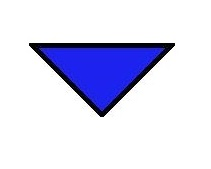
\includegraphics[scale=0.1, angle=180, origin=c]{independentKnowledgeable.png}
		IndependentKnowledgeable &
		\begin{tabular}{@{}lll@{}}
			 [50, 100] & \hspace{.8cm} [50, 100] \end{tabular}\\ \midrule 
		 \rowcolor[HTML]{FFFFFF} 
		 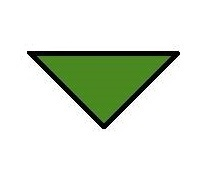
\includegraphics[scale=0.1, angle=180, origin=c]{independentUnknowledgeable.png}
		 IndependentUnknowledgeable &
		 \begin{tabular}{@{}lll@{}}
		 	[50, 100] & \hspace{.8cm} [0, 50] \end{tabular}\\ \midrule 
	 	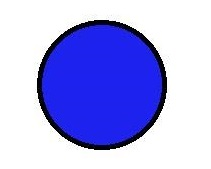
\includegraphics[scale=0.1, angle=180, origin=c]{dependentKnowledgeable.png}
		 DependentKnowledgeable &
		 \begin{tabular}{@{}lll@{}}
		 	[0, 50] & \hspace{1.2cm} [50, 100] \end{tabular}\\ \midrule 
	 			 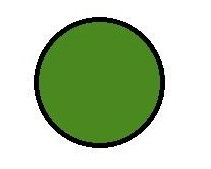
\includegraphics[scale=0.1, angle=180, origin=c]{dependentUnknowledgeable.png}
		DependentUnknowledgeable &
 		\begin{tabular}{@{}lll@{}}
 			[0, 50] & \hspace{1.2cm} [0, 50] \end{tabular}\\ \midrule 
	\end{tabular}
	\caption{Diferentes tipos de agente, de acordo com os valore possíveis para os atributos considerados.}
\end{table}

Esta classificação permitiu a definição, ao nível de interface, de diferentes representações para os vários tipos de agente, permitindo estabelecer visualmente a relação entre o tipo de agente e os seus comportamentos.

\setlength{\tabcolsep}{20pt}
\renewcommand{\arraystretch}{1.3}
\begin{table}[H]
	\centering
	\label{agent-behaviours}
	\begin{tabular}{@{}lll@{}}
		\toprule
		\rowcolor[HTML]{FFFFFF} 
		\textbf{Comportamento}  & \textbf{Descrição}                                                                                                                                   \\ \toprule
		\rowcolor[HTML]{FFFFFF} 
		\begin{tabular}[c]{@{}l@{}}Processo de\\Evacuação\end{tabular} & \begin{tabular}[c]{@{}l@{}}A cada momento um agente deve usar o seu\\conhecimento da área e mover-se em direção à saída.\end{tabular}  \\ \midrule 
		\rowcolor[HTML]{FFFFFF} 
	    \begin{tabular}[c]{@{}l@{}}Mecanismo de\\Pânico\end{tabular} & \begin{tabular}[c]{@{}l@{}}A cada momento um agente atualiza o seu estado\\ de pânico de acordo com a sua condição e o\\ambiente envolvente.\end{tabular}  \\ \midrule 
	    \rowcolor[HTML]{FFFFFF} 
	    \begin{tabular}[c]{@{}l@{}}Sentido de\\Altruísmo\end{tabular} & \begin{tabular}[c]{@{}l@{}}A cada momento um agente monitoriza o ambiente\\ envolvente e decide responder ou ignorar pedidos de\\ ajuda de outros agentes.\end{tabular}  \\ \midrule 
	    \rowcolor[HTML]{FFFFFF} 
	    \begin{tabular}[c]{@{}l@{}}Pedido de\\Direções\end{tabular} & \begin{tabular}[c]{@{}l@{}}Um agente toma, por ser pouco independente ou ter\\ pouco \\conhecimento da área, pede direções a agentes\\ na sua proximidade.\end{tabular}  \\ \midrule 
	    \rowcolor[HTML]{FFFFFF} 
	    \begin{tabular}[c]{@{}l@{}}Pedido de\\Ajuda\end{tabular} & \begin{tabular}[c]{@{}l@{}}Um agente incapaz de se mover de forma autónoma\\ pede ajuda aos agentes na sua proximidade.\end{tabular}  \\ \midrule 
		                                                       
	\end{tabular}
		\caption{Comportamentos dos agentes.}
\end{table}

\subsection{Interações}

A comunicação entre agentes foi implementada recorrendo a mensagens \textit{JADE}, obedecendo aos protocolos \textit{FIPA}. 

Dado que todos os agentes se encontram, a cada momento, numa dada posição de um espaço, cada agente pode tomar conhecimento daqueles que o rodeiam, sendo possível obter os seus \textit{AID}’s usando a noção de proximidade.\newline

\renewcommand{\lstlistingname}{Excerto}

\begin{lstlisting}[caption= Código \textit{Java}\, ilustrando a possibilidade de uma pessoa poder descobrir outras.]
// find people in the surrounding area
ArrayList<AID> peopleNear = environment.findNear(myAgent);
if(peopleNear.isEmpty()) {
	return;
}
\end{lstlisting}

\paragraph{}

Os vários agentes assumem uma atitude mais ou menos cooperativa, em função dos atributos altruísmo e independência, e partilham um objetivo comum: chegar a uma saída.
\newline

Com vista a simular de forma algo fidedigna as condições de uma evacuação de emergência, foram implementadas as seguintes interações entre agentes:

\begin{itemize}

\item Terror;

Um agente cujo nível de pânico sobe acima de um certo nível envia uma mensagem \textit{PROPAGATE} para agentes na proximidade.

Aqueles que recebem esta mensagem, podem, ou não, propagar a mensagem e aumentam o seu estado de pânico - variação que depende de diversos fatores: assumiu-se que as pessoas mais independentes são menos influenciáveis pelos gritos dos outros enquanto os mais jovens ou mais idosos são mais impressionáveis.\newline



\begin{figure}[H]
	\centering
	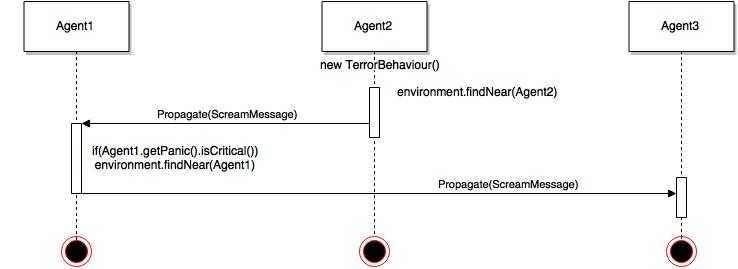
\includegraphics[scale=0.5]{terror-behaviour.jpg}
	\caption{Diagrama de sequência exemplificando uma interação do tipo Terror.}
	\label{uml}
\end{figure}

\item Orientação;

Duas pessoas podem partilhar conhecimento sobre a área, mediante um pedido nesse sentido. Um agente que tenha pouco conhecimento da área pode enviar a um agente ao seu redor uma mensagem \textit{CFP}, a que esse agente responde com uma dada probabilidade - dependente do valor do atributo altruísmo. A resposta consiste numa mensagem \textit{INFORM}, com o valor do seu conhecimento da área, \textit{conhecimento1}. Por forma a simular a aquisição de informação, o agente que fez o pedido atualizará o seu nível de conhecimento da área, \textit{conhecimento2}, de acordo com:

\[	conhecimento2 = max(conhecimento2, conhecimento1 * FAC) \]

onde FAC representa um fator de aquisição de conhecimento, de valor configurável, que visa simular as perdas de informação típicas numa troca de informações.\newline

\begin{figure}[H]
	\centering
	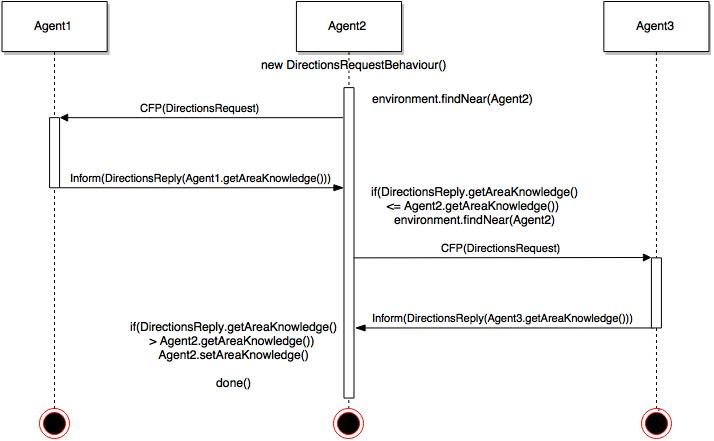
\includegraphics[scale=0.5]{directions-behaviour.jpg}
	\caption{Diagrama de sequência exemplificando uma interação do tipo Orientação.}
	\label{uml}
\end{figure}
\newpage


\item Ajuda.

Um agente pode pedir ajuda, enviando uma mensagem \textit{CFP} para agentes ao seu redor. Os agentes na disposição de ajudar podem oferecer a sua ajuda, enviando uma mensagem \textit{PROPOSAL}, com o valor da sua mobilidade, \textit{mobilidade1}.

O autor do pedido de ajuda aceita a melhor oferta, respondendo com uma mensagem \textit{ACCEPT\_PROPOSAL}, com o valor da sua mobilidade, \textit{mobilidade2}, rejeitando as demais ofertas com uma mensagem \textit{REJECT\_PROPOSAL}. O agente que ofereceu ajuda passa a guiar o outro até à saída, sendo a mobilidade de cada um dada por:

\[	mobilidade1 = mobilidade2 = \frac{mobilidade1 + moblidade2}{2} \]\newline

\begin{figure}[H]
	\centering
	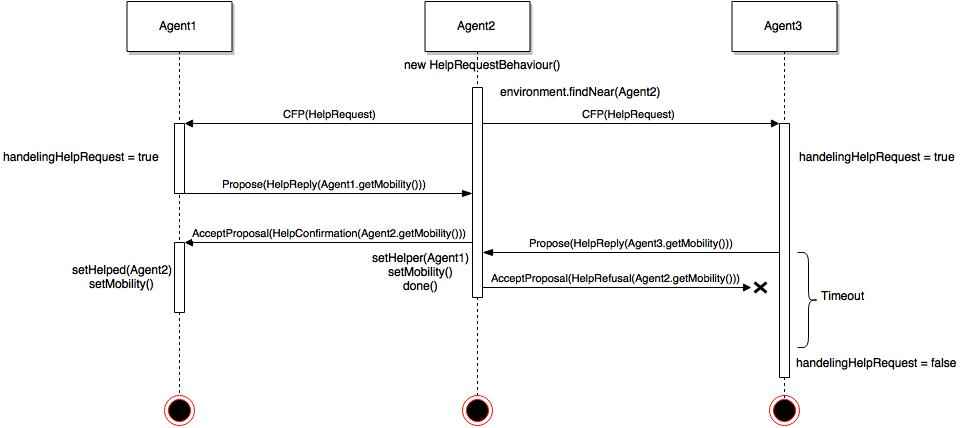
\includegraphics[scale=0.45]{help-behaviour.jpg}
	\caption{Diagrama de sequência exemplificando uma interação do tipo Ajuda.}
	\label{uml}
\end{figure}

\end{itemize}

Como pode constatar-se, estes protocolos são relativamente simples. De referir, ainda, que as interações Ajudar e Orientar são efetuadas de acordo com o modelo de Rede Contratual, sendo que, no caso, o papel de gestor cabe ao agente que faz o pedido inicial. 


%----------------------------------------------------------------------------------------
%	DESENVOLVIMENTO
%----------------------------------------------------------------------------------------

\newpage
\section{Desenvolvimento}
\subsection{Faseamento}
A implementação do projeto executou-se em diferentes etapas:
\begin{enumerate}
	\item Especificação e planeamento (23 de outubro a 1 de novembro);
	\item Implementação de:
	 \begin{enumerate} 
	 	\item Agente (25 de outubro a 5 de novembro);
	 	\item Espaço (5 de novembro a 25 de novembro);
	 	
	 	Teste e análise do comportamento de um agente num espaço.
		\item Interação entre agentes (5 de novembro a 5 de dezembro);
		
		Teste e análise do comportamento de vários agentes num espaço. 
	\end{enumerate}
	\item Exploração de diferentes cenários e recolha e avaliação de métricas (1 de dezembro a 10 de dezembro).
\end{enumerate}

\subsection{Ambiente de Desenvolvimento e Ferramentas}
O desenvolvimento decorreu em ambiente \textit{Windows} 10 e usando a versão \textit{Neon} do \textit{IDE Eclipse}, tendo-se feito uso das ferramentas \textit{JADE}, \textit{Repast Simphony} e \textit{SAJaS}.
\newline

\textbf{\textit{JADE}:} Definição de agentes.

\textbf{\textit{Repast Simphony}:} Simulação multiagente.

\textbf{\textit{SAJaS}:} Integração de agentes \textit{JADE} com \textit{Repast}.
\newline

O \textit{Repast} é uma \textit{framework open-source} que permite criar, analisar e experimentar com mundos artificiais populados por agentes que interagem de forma não trivial.

Concretamente, utilizou-se a sua mais recente versão - \textit{Repast Simphony}, que permite programar em \textit{Java} a estrutura espacial, a estrutura lógica e os comportamentos dos agentes.

Tem sido amplamente utilizado em aplicações de simulação, e, no caso, considerou-se de particular utilidade, por um lado, a capacidade de definir e lidar com estruturas espaciais e, por outro, a recolha de métricas associadas às simulações realizadas. Por último, tem-se a vantagem de poder acompanhar, de forma visual, o decorrer da simulação.

Adicionalmente, utilizou-se a \textit{API SAJaS}, que possibilitou a integração de agentes \textit{JADE} com \textit{Repast}, permitindo definir os comportamentos de agentes e fazer uso das capacidades de comunicação entre agentes, visando simular as interações expectáveis num cenário de evacuação.

\subsection{Estrutura}

A aplicação pode, a nível lógico, dividir-se em diferentes módulos, com responsabilidades distintas.
\begin{figure}[H]
	\centering
	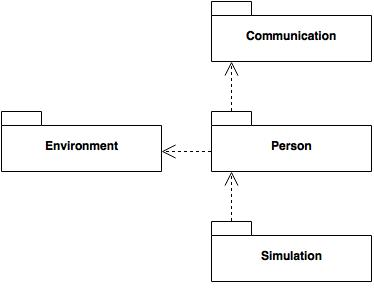
\includegraphics[scale=0.8]{packages.jpg}
	\caption{Diagrama ilustrativo da estrutura lógica do projeto.}
	\label{uml}
\end{figure}

O módulo \textit{Simulation} é responsável, por um lado, pela configuração da simulação, no que diz respeito às ferramentas usadas - \textit{Repast}, \textit{JADE} e \textit{SAJaS} -, e, por outro lado, pela definição do cenário da simulação - tanto o espaço como a população a evacuar. 

Adicionalmente, inclui a componente de recolha de estatísticas da simulação - \textit{ResultsCollector} -, implementado como um agente, cuja função é receber dados relativos à evacuação de cada uma das pessoas evacuadas.

\begin{figure}[H]
	\centering
	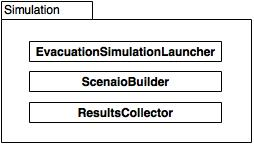
\includegraphics[scale=0.8]{simulation.jpg}
	\caption{Classes do módulo \textit{Simulation}.}
	\label{uml}
\end{figure}
\newpage
O módulo \textit{Environment} contempla tudo o que se relaciona com a definição da estrutura espacial da simulação, bem como a sua configuração.\newline

\begin{figure}[H]
	\centering
	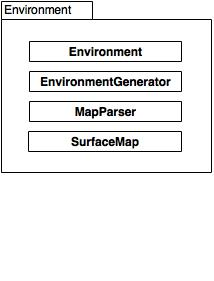
\includegraphics[scale=0.6]{environment.jpg}
	\caption{Classes do módulo \textit{Environment}.}
	\label{uml}
\end{figure}

O módulo \textit{Person} é formado pela classe \textit{Person} - subclasse de \textit{Agent} e onde são definidos os atributos e comportamentos de uma pessoa -, bem como as suas várias subclasses.

\begin{figure}[H]
	\centering
	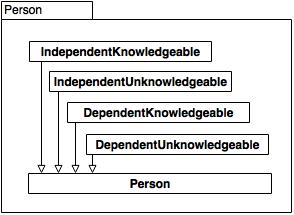
\includegraphics[scale=0.8]{person.jpg}
	\caption{Classes do módulo \textit{Person}.}
	\label{uml}
\end{figure}
\newpage
O módulo \textit{Communiation} é formado pelas classes usadas na implementação da comunicação entre agentes. Estas classes são tipos de mensagens trocadas em interações entre agentes, e caracterizam a \textit{SimulationOntology}.

\begin{figure}[H]
	\centering
	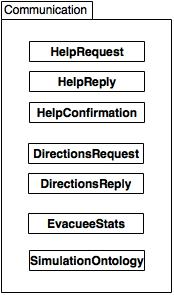
\includegraphics[scale=0.7]{communication.jpg}
	\caption{Classes do módulo \textit{Communication}.}
	\label{uml}
\end{figure}

\begin{figure}[H]
	\centering
	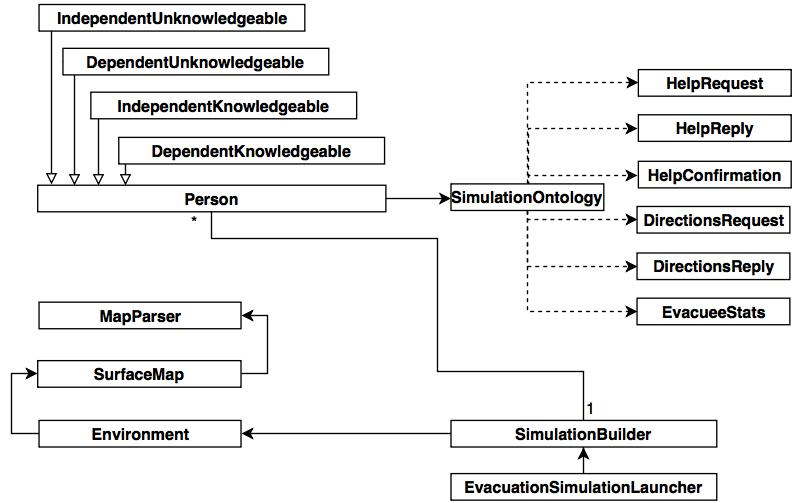
\includegraphics[scale=0.5]{classes.jpg}
	\caption{Diagrama de classes do projeto (simplificado).}
	\label{uml}
\end{figure}


\newpage
\subsection{Detalhes de Implementação}
\subsubsection{Agentes}

\begin{itemize}
	
\item \textbf{Atributos}

Conforme descrito na especificação, os agentes encontram-se definidos por um conjunto de atributos.
Na definição da variação de alguns dos atributos usados, partiu-se de alguns pressupostos:

\begin{itemize}
\item Pânico

Assumiu-se que o pânico de uma pessoa pode aumentar - por exemplo, como resultado de um empurrão - ou diminuir - por exemplo, quando recebe ajuda por parte de outra pessoa. 

Mais ainda, tem-se que o pânico aumenta mais depressa do que diminui e, no cálculo dessa variação considerou-se que as pessoas mais independentes têm uma reação mais moderada, i.e., veem o seu nível de pânico variar de forma mais comedida. Pelo contrário, jovens e pessoas de idade mais avançada reagem de forma mais pronunciada, isto é, veem o seu nível de pânico variar de forma errática.

Numa tentativa de aproximar a simulação daquilo que seria observável numa situação real, considerou-se que o pânico condiciona a capacidade de uma pessoa usar o seu conhecimento da área e escolher um caminho até à saída. Por outro lado, fez-se igualmente depender do estado de pânico de uma pessoa a probabilidade de empurrar alguém que se encontre no caminho que pretende seguir.\newline


\item Mobilidade

No que diz respeito à mobilidade, consideram-se apenas variações negativas - por exemplo, provocadas por empurrões -, sendo que aquelas mais jovens ou de idade mais avançada verão a sua mobilidade diminuir de forma mais rapidamente.

Não obstante, a mobilidade de uma pessoa pode ser temporariamente aumentada, sempre que uma pessoa for ajudada por outra. Se, por motivo de empurrão ou morte, essa ajuda terminar, a mobilidade da pessoa é restaurada para o seu valor anterior.

Da mobilidade de uma pessoa depende a probabilidade de, a cada instante, uma pessoa se mover. A mobilidade constringe, ainda, o altruísmo de uma pessoa, limitando a resposta a pedidos de ajuda recebidos.\newline

\item Conhecimento da área

O conhecimento da área pode variar, aumentando apenas por meio da partilha de informação com outras pessoas.

O conhecimento da área condiciona a probabilidade de um agente de, a cada instante, selecionar o melhor caminho na direção da saída.\newline

\item Paciência

Considerou-se que a paciência de uma pessoa oscila, aumentando - por exemplo, quando o agente vê o seu caminho escolhido obstruído por outro agente - ou diminuindo - por exemplo, quando o agente consegue mover-se com sucesso - de acordo com um valor predefinido e configurável.

A paciência de uma pessoa influencia a forma como o caminho a seguir é selecionado: se o caminho selecionado estiver bloqueado por outra pessoa e não se quiser empurrá-la, pode esperar-se por um tempo razoável, até que essa pessoa desobstrua a passagem (reduzindo a paciência a cada tentativa de movimento), ou, esgotada a paciência, escolher um outro caminho disponível.

\end{itemize}

Adicionalmente, definiram-se algumas funções, que traduzem a influência do pânico sobre outros atributos:

\begin{lstlisting}[caption= Código \textit{Java}\ de funções que traduzem a influência do pânico sobre o altruísmo e cohecimento de área.]
public int getAltruisticFeeling() {
	return altruism - panic / 5;
}

public int getUsableKnowledge() {
	return areaKnowledge - panic / 5;
}
\end{lstlisting}

De referir que, para todos os atributos, sempre que é feita uma atribuição - por meio do uso de um método \textit{setAtributo(novoValor)}, o valor desse atributo é atualizado para o novo valor apenas se respeitar os limites definidos.
\newline
\begin{lstlisting}[caption= Código \textit{Java}\ da função que assegura que os vários atributos respeitam os limites definidos.]
int enforceBounds(int attribute) {
	if(attribute > MAX_SCALE){
		return MAX_SCALE;
	}else if(attribute < MIN_SCALE){
		return MIN_SCALE;
	}else{
		return attribute;
	}
}
\end{lstlisting}
\newpage

\item \textbf{Mecanismo de Pânico}

Pela especificação, um agente cujo nível de pânico sobe acima de um certo nível envia uma mensagem \textit{PROPAGATE} para agentes na proximidade, sempre que atualiza o seu nível de pânico.

\begin{lstlisting}[caption= Código \textit{Java}\ responsável pelo envio de um grito.]
ACLMessage msg = receive(template);
if(msg!= null) {
	if(msg.getContent().equals(SCREAM_MESSAGE)){
		increasePanic();
	}
}
\end{lstlisting}

Aqueles que recebem esta mensagem, podem, ou não, propagar a mensagem e aumentam o seu estado de pânico - variação que depende de diversos fatores: assumiu-se que as pessoas mais independentes são menos influenciáveis pelos gritos dos outros enquanto os mais jovens ou mais idosos são mais impressionáveis.\newline


\item \textbf{Partilha de Direções}

Conforme a especificação, duas pessoas podem partilhar conhecimento sobre a área, mediante um pedido nesse sentido. 

A cada instante, um agente que tenha pouco conhecimento da área pode - com uma probabilidade inversamente proporcional a esse conhecimento - enviar a um agente ao seu redor uma mensagem \textit{CFP}.

\begin{lstlisting}[caption= Código \textit{Java}\ da função responsável pelo envio de um pedido de direções.]
boolean sendDirectionsRequest() {
	ArrayList<AID> peopleNear = environment.findNearAgents(myAgent, REQUEST_DISTANCE);
	peopleNear.removeAll(previousReplies);
	SimUtilities.shuffle(peopleNear,  RandomHelper.getUniform());
	if(peopleNear.isEmpty()) {
		return false;
	}
	
	ACLMessage directionsRequest = new ACLMessage(ACLMessage.CFP);			
	directionsRequest.addReceiver(peopleNear.get(0));
	DirectionsRequest requestMessage = new DirectionsRequest();
	getContentManager().fillContent(directionsRequest, requestMessage);
	send(directionsRequest);
	
	return true;
}
\end{lstlisting}

O agente a quem foram pedidas direções responde com uma mensagem \textit{INFORM} ou \textit{REFUSE}, com uma dada probabilidade, associada ao seu altruísmo.

\begin{lstlisting}[caption= Código \textit{Java}\ da função responsável pela receção de pedidos de direções.]
void handleDirectionsRequest(ACLMessage request) {
	ACLMessage reply = request.createReply();
	
	if(RandomHelper.nextIntFromTo(MIN_SCALE, MAX_SCALE) < getAltruisticFeeling()) {
		reply.setPerformative(ACLMessage.INFORM);
	}else{
		reply.setPerformative(ACLMessage.REFUSE);
	}
	
	DirectionsReply replyMessage = new DirectionsReply(areaKnowledge);
	getContentManager().fillContent(reply, replyMessage);
	send(reply);
}
\end{lstlisting}

O agente que pediu direções atualiza o seu conhecimento da área.

\begin{lstlisting}[caption= Código \textit{Java}\ da função responsável pela receção de respostas a um pedido de direções.]
void receiveReply() {
	ACLMessage msg = receive(template);
	if(msg == null) {
		return;
	}
	
	if(msg.getPerformative() == ACLMessage.INFORM) {				
		int previousKnowledge = areaKnowledge;
		int knowledgeReceived = ((DirectionsReply) getContentManager().extractContent(msg)).getKnowkledge();
		
		setAreaKnowledge(Integer.max((int) (knowledgeReceived * KNOWLEDGE_ACQUISITION_FACTOR), areaKnowledge));
		
		if(previousKnowledge < areaKnowledge){
			newDirections = true;
		}else{
			previousReplies.add(msg.getSender());
		}
	}else if(msg.getPerformative() == ACLMessage.REFUSE){			
		newDirectionsRequested = false;
	}
}
\end{lstlisting}
\item \textbf{Ajuda}

Seguindo a especificação, uma pessoa com mobilidade reduzida pode pedir ajuda a outra na sua proximidade. 

A cada instante, um agente que tenha pouca mobilidade da área pode - com uma probabilidade inversamente proporcional a essa mobilidade - enviar aos agentes ao seu redor uma mensagem \textit{CFP}.

\begin{lstlisting}[caption= Código \textit{Java}\ de envio de um pedido de ajuda.]
boolean sendRequest() {
	ArrayList<AID> peopleNear = environment.findNearAgents(myAgent);
	if(peopleNear.isEmpty()) {
		return false;
	}

	ACLMessage helpRequest = new ACLMessage(ACLMessage.CFP);
	for(AID person : peopleNear)
		helpRequest.addReceiver(person);
	
	helpRequest.setLanguage(codec.getName());
	helpRequest.setOntology(serviceOntology.getName());
	
	HelpRequest requestMessage = new HelpRequest();
	getContentManager().fillContent(helpRequest, requestMessage);
	send(helpRequest);
	
	return true;
}
\end{lstlisting}

Os agentes a quem foi pedida ajuda respondem com uma mensagem \textit{ACCEPT\_PROPOSAL} ou \textit{REJECT\_PROPOSAL}, com uma dada probabilidade, associada ao seu altruísmo.

\begin{lstlisting}[caption= Código \textit{Java}\ da função responsável pela receção de pedidos de direções.]
void handleHelpRequest(ACLMessage request){
	if((helped != null || handlingHelpRequest) && RandomHelper.nextIntFromTo(MIN_SCALE, MAX_SCALE) < getAltruisticFeeling() 
	&& getMobility() > getMobilityHelpResponseThreshold()) {
		ACLMessage reply = request.createReply();
		reply.setPerformative(ACLMessage.PROPOSE);			
		HelpReply replyMessage = new HelpReply(mobility, areaKnowledge);
		getContentManager().fillContent(reply, replyMessage);
		send(reply);
	}
}
\end{lstlisting}

O agente que pediu ajuda regista as propostas, e, após algum tempo, seleciona a melhor das propostas e envia uma confirmação.

\begin{lstlisting}[caption= Código \textit{Java}\ das funções responsáveis pela receção e confirmação de prospostas de ajuda.]
boolean receiveReplies() {
	ACLMessage msg = receive(template);
	
	if(msg != null) {
		HelpReply proposal = (HelpReply) getContentManager().extractContent(msg);
		proposal.setProposerAID(msg.getSender());
		proposals.add(proposal);
	}else{
		nAttempts++;
	}
	return nAttempts < MAX_ATTEMPTS;
}

void acceptBestProposal() {
	proposals.sort();
	HelpReply bestProposal = proposals.get(0);
	proposals.remove(bestProposal);
	
	ACLMessage msg = new ACLMessage(ACLMessage.ACCEPT_PROPOSAL);
	msg.addReceiver(bestProposal.getProposerAID());
	msg.setLanguage(codec.getName());
	msg.setOntology(serviceOntology.getName());
	HelpConfirmation confirmationMessage = new HelpConfirmation(mobility, areaKnowledge);
	getContentManager().fillContent(msg, confirmationMessage);
	send(msg);
	decreasePanic();
	
	Person helper = environment.findAgent(bestProposal.getProposerAID());
	setHelper(helper);
	shareMobility(bestProposal.getMobility());		
	setAreaKnowledge(Integer.max(areaKnowledge, bestProposal.getAreaKnowledge()));
	
	if(!proposals.isEmpty()) {
		msg.setPerformative(ACLMessage.REJECT_PROPOSAL);
		for(HelpReply proposal: proposals) {
			msg.addReceiver(proposal.getProposerAID());
		}
		send(msg);
	}
}
\end{lstlisting}

\item \textbf{Empurrões}

No contexto do problema, designou-se por «empurrão» a interação entre duas pessoas em que uma das pessoas, ao tentar mover-se, tem alguém à sua frente e decide removê-la do seu caminho à força, «empurrando-a».

Na circunstância de o caminho selecionado se encontrar obstruído, um agente pode - conforme o seu estado de pânico ou impaciência - «empurrar» o agente que está a provocar esse bloqueio.

Efetivamente, o «empurrão» consiste na troca de posições entre dois agentes. O agente que é «empurrado» vê a sua mobilidade reduzida e o seu nível de pânico aumentar.
Se o agente empurrado estiver a ajudar ou a ser ajudado por outro, essa relação de ajuda é terminada.

\begin{lstlisting}[caption= Código \textit{Java}\, da função que permite a uma pessoa «empurrar» outra.]
void push(int selectedX, int selectedY) {
	Person person = environment.userInCell(selectedX, selectedY);
	if(person == null || (selectedX == x && selectedY == y)){
		return;
	}
	
	boolean isPush = helped!=null ? !person.getAID().equals(helped.getAID()) : true;	
	if(isPush){
		if(person.getHelper() != null){
			person.getHelper().setHelpee(null);
			setHelper(null);
		}else{
			if(person.getHelpee() != null){
				person.getHelpee().setHelper(null);
				setHelpee(null);
			}	
			person.increasePanic();
		}	
		person.decreaseMobility();
	}			
	
	if(RandomHelper.nextIntFromTo(MIN_SCALE, MAX_SCALE) > altruism) {
		person.decreasePatience();
	}
	
	person.moveTo(x, y);
	moveTo(selectedX, selectedY);
}
\end{lstlisting}

De notar que, para esta interação, não existe troca de mensagens entre os agentes, por se considerar esta aproximação mais próxima do que seria observável numa situação real.

\item \textbf{Movimento}
(TODO)


\end{itemize}

\subsubsection{Ambiente}
A representação do espaço é feita com recurso a múltiplas estruturas de dados, designadamente, uma \textit{Grid} - classe disponibilizada pelo \textit{Repast} - que contém os agentes, um \textit{array} bidimensional de caracteres com as posições das saídas e das paredes/obstáculos e um \textit{array} bidimensional de inteiros com um mapa de distâncias. 

Um utilizador tem a liberdade de indicar, na interface da simulação, um ficheiro com a configuração do ambiente onde estarão necessariamente definidas as posições das saídas e das paredes/obstáculos.

\begin{itemize}

\item \textbf{Mapa de obstáculos e saídas}

Este mapa é representado como um \textit{array} bidimensional com caracteres que representam as saídas, paredes/obstáculos ou espaços livres, nas posições em que estão definidas no ficheiro de configuração. Esta representação é usada tanto para a criação do mapa de distâncias como para determinar,em \textit{runtime}, se uma célula contem um obstáculo ou uma saída.

\begin{figure}[H]
	\centering
	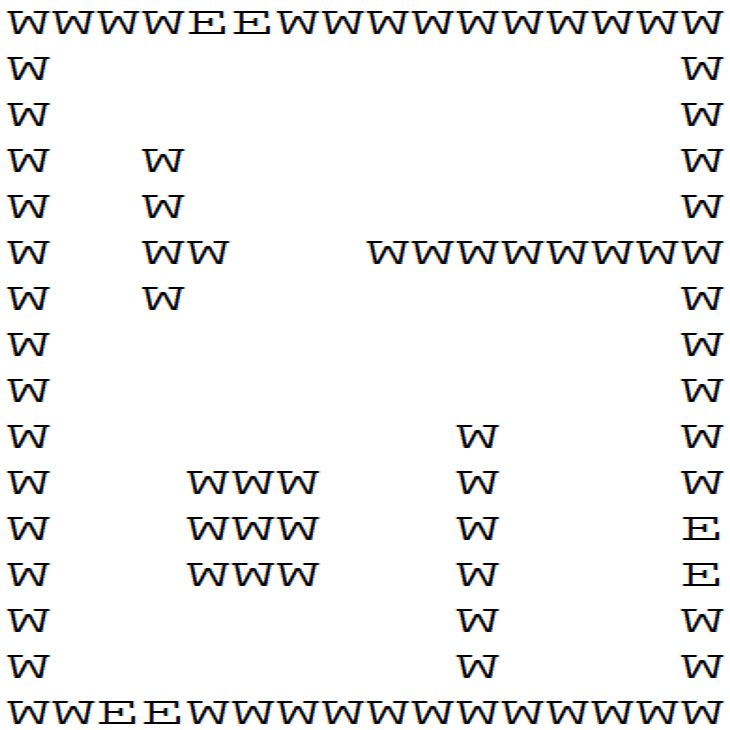
\includegraphics[scale=0.2]{map_text.png}
	\caption{Representação visual do conteúdo do mapa de obstáculos e saídas.}
	\label{map}
\end{figure}

\item \textbf{Mapa de distâncias}

Antes da execução da simulação, no momento em que o mapa é carregado, é construído um mapa com as distâncias até às saídas. 

Este é obtido usando um algoritmo, semelhante a \textit{flooding}, que, começando a partir de cada saída, se propaga, colocando o valor atual de distância a essa saída nas células, parando de se propagar num certo sentido caso encontre uma célula já preenchida com um valor inferior ao valor que seria colocado ou caso encontre um obstáculo.
\newpage
\begin{lstlisting}[caption= Pseudo-código do algoritmo usado para o preenchimento do mapa de distâncias.]
generateDistanceMap() {
	distanceMap; // Mapa de distancias

	for(exit in exitsList){
		distance = 1;
		toVisit; 		// Array com celulas a visitar
		visited; 		// Array com celulas ja visitadas
		futureToVisit; 	// Array com celulas a ser visitadas no futuro
		toVisit.add(exit);

		while( !toVisit.empty() ) {

			for(cell in toVisit){
				
				for(cardinal in cardinalPoints){		// Por cada ponto cardeal ver celula adjacente
					if(cell.cardinal == ' ' and !visited.contains(cell.cardinal)){ // Verifica se a celula adjacente corresponde a um espaco livre e ainda nao foi visitada
						if(distance < distanceMap.get(cell.cardinal)){ // Se a distancia atual for mais baixa que a distancia que a celula ja tinha
							futureToVisit.add(cell.cardinal);
							distanceMap.set(cell.cardinal, distance);
						}
						visited.add(cell.cardinal);
					}
				}
			}
			toVisit = futureToVisit;
			futureToVisit.clear();
			distance++;
		}
	return distanceMap;		
}
\end{lstlisting}

Este pré-processamento do melhor caminho até à saída mais próxima, a partir de cada célula, é uma abordagem válida, tendo em conta que se considerou o ambiente como sendo estático. Revela também ter um desempenho consideravelmente melhor do que se fosse usado um algoritmo de \textit{path finding} a cada tentativa de movimento. 

\begin{figure}[H]
	\centering
	\includegraphics[scale=0.5]{map_distance.png}
	\caption{Representação visual do conteúdo do mapa de distâncias\protect\footnotemark.}
	\label{map}
\end{figure}

\footnotetext{Nota: Cores usadas meramente com o propósito de facilitar a compreensão da figura. Na representação do mapa de distâncias não há nenhuma indicação explícita de qual é a saída mais próxima, essa informação é extraída a partir dos valores nas células vizinhas. \\Apesar de não ser apresentado na figura, as paredes contém valor -1.}

\item \textbf{\textit{Grid}}

Para o ambiente ter uma representação visual na interface de simulação, é necessário o uso de uma \textit{Grid}, sendo que esta contém todos os agentes, obstáculos e saídas.

A \textit{Grid} permite que um agente conheça a sua vizinhança, tornando possível usar a próximidade física entre agentes como um factor para os comportamentos entre estes. É também através desta \textit{Grid} que se pode observar o movimento dos agentes pelo espaço, contornando obstáculos e tentando atingir as saídas.

\begin{figure}[H]
	\centering
	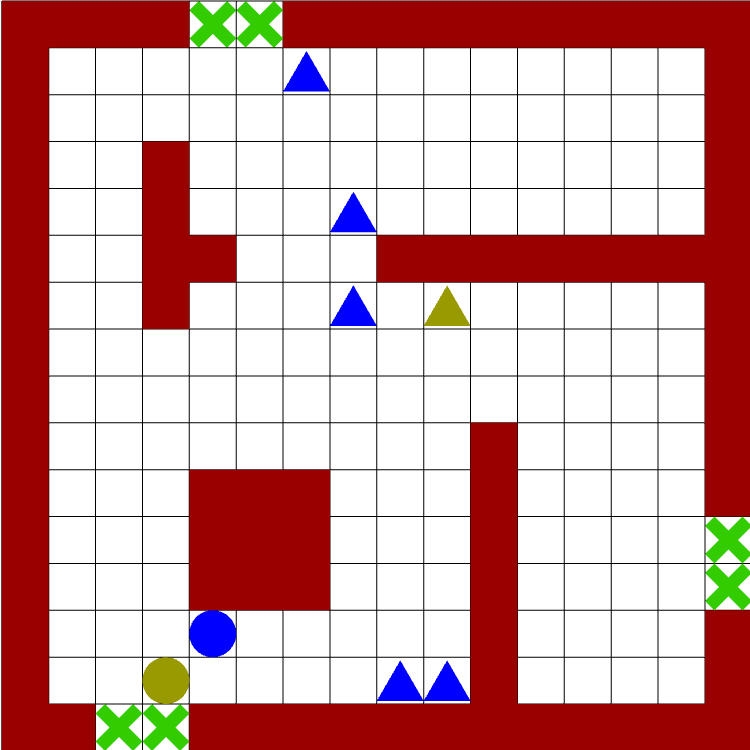
\includegraphics[scale=0.20]{map_simulation.png}
	\caption{Representação da \textit{Grid} na interface da simulação}
	\label{map}
\end{figure}

\end{itemize}

\newpage
\section{Experimentação}

Ao longo do processo de desenvolvimento foram levadas a cabo múltiplas experiências, com vista a testar a implementação dos agentes.
\begin{itemize}
	
%----------------------------------------------------------------------------------------
%	EXP begin
%----------------------------------------------------------------------------------------
	
\item \textbf{Evacuação simples}

\textbf{Objetivo:} 
                                                                                                                                  	Testar se um agente é capaz de atingir a saída.
	
Esta experiência consistiu na colocação, numa dada posição de um espaço pré-definido, de um agente de um certo tipo, tendo-se analisado o seu comportamento e medido o tempo que decorreu até que chegassem à saída.
	
\setlength{\tabcolsep}{20pt}
\renewcommand{\arraystretch}{1.3}
\begin{table}[H]
	\centering
	\caption{Tempos de evacuação em função do tipo de agente usado.}
	\begin{tabular}{@{}lll@{}}
		\toprule
		\rowcolor[HTML]{FFFFFF} 
		\textbf{Tipo de agente}  & \textbf{Tempo de evacuação}\\
		\toprule
		\rowcolor[HTML]{FFFFFF} 
		IndependentKnowledgeable & 16.73s \\ \midrule 
		\rowcolor[HTML]{FFFFFF} 
		IndependentUnknowledgeable & 34.79s \\ \midrule 
		DependentKnowledgeable & 17.71s \\ \midrule 
		DependentUnknowledgeable &
		50.12s \\ \midrule 
	\end{tabular}
\end{table}
	
	Como esperado, observou-se que os agentes com maior conhecimento da área demoraram menos tempo a chega à saída.
	
	Dado que, nesta fase, se utilizou apenas um agente de cada tipo em cada simulação, o atributo independência não se reflete no desempenho do agente, tendo-se observado tempos de evacuação semelhantes para os agentes dos tipos \textit{IndependentKnowledgeable} e \textit{DependentKnowledgeable}. 
	
	O mesmo não foi observado no caso dos agentes de tipos \textit{DependentKnowledgeable} e \textit{DependentUnknowledgeable}, devido ao caráter estocástico das simulações.

	%----------------------------------------------------------------------------------------
	
	\item \textbf{Mecanismo de pânico}
	
	\textbf{Objetivo:} 
	Testar o mecanismo de pânico.
	
	Esta experiência consistiu na colocação, em posições adjacentes de um espaço pré-definido, de dois agentes, sendo que um deles caracterizado por um elevado nível de pânico. No caso, ambos os agentes são do tipo \textit{IndependentKnowledgeable}, embora tal não seja relevante para o objetivo desta experiência, podendo, de facto, ter-se usado agentes de qualquer um dos tipos definidos.
	
	Procedeu-se à análise dos seus comportamentos e, no final, verificaram-se os seus níveis de pânico. 
		Como esperado, observou-se que um agente em pânico «emite um grito», conforme a especificação deste tipo de interação. O outro agente «ouve o grito» e aumenta o seu nível de pânico - como se pode observar na Figura \ref{panic_log}.
	
	\begin{figure}[H]
		\centering
		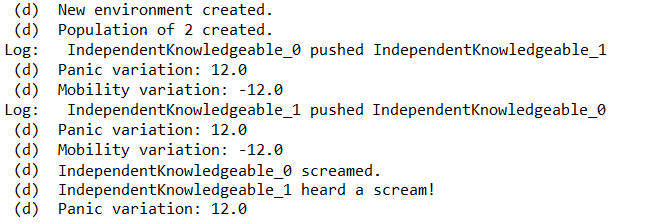
\includegraphics{panic_log.png}
		\caption{Excerto do registo de execução de uma simulação do cenário descrito.}
		\label{panic_log}
	\end{figure}

	Em algumas das execuções, como nesta, observaram-se «empurrões», devido ao facto de se encontrarem em posições adjacentes e ao facto de os agentes estarem num estado de pânico. 
	
	No caso, um dos agentes «empurrou» o outro, o que produziu o primeiro aumento do nível de pânico, visível no gráfico da Figura \ref{panic_graph}. 
	
	Seguiu-se um novo «empurrão», desta vez, por parte do agente que tinha sido «empurrado» antes, causando um novo aumento do nível de pânico. 
	
	O terceiro aumento do pânico observado fica a dever-se ao «grito» que o agente em pânico lançou ao ser empurrado, e reflete a reação do agente que o empurrou a esse mesmo «grito». 
	
	\begin{figure}[H]
		\centering
		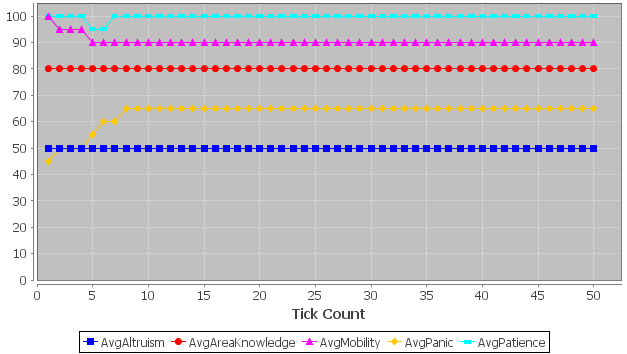
\includegraphics{panic_test.png}
		\caption{Variação dos atributos dos agentes do cenário.}
		\label{panic_graph}
	\end{figure}
	
	Salienta-se, ainda, a diminuição da mobilidade verificada a cada «empurrão», observável na Figura \ref{panic_graph}.\newline
	
	
	%----------------------------------------------------------------------------------------
		
	\item \textbf{Pedido de direções}
	
	\textbf{Objetivo:} 
	Testar a partilha de conhecimento entre dois agentes.
	
	Esta experiência consistiu na colocação, em posições adjacentes de um espaço pré-definido, de um agente do tipo \textit{IndependentKnowledgeable}, com um elevado nível de altruísmo, e de um agente do tipo \textit{DependentUnknowledgeable}, com um conhecimento da área reduzido.
	
	\begin{figure}[H]
	\centering
	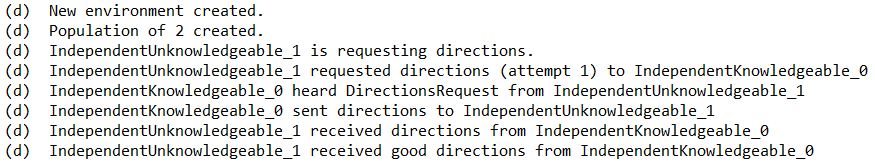
\includegraphics[scale=.8]{directions_log.png}
	\caption{Excerto do registo de execução de uma simulação do cenário descrito.}
	\label{directions_log}
	\end{figure}

	Confirmou-se que o agente com menor conhecimento da área efetuou um pedido de direções, que despoleta uma resposta por parte do outro agente. Recebendo esta resposta, o agente que efetuou o pedido atualiza o seu conhecimento da área com base na informação que contém e num fator de aquisição de conhecimento, como detalhado. Na Figura \ref{directions_graph} é possível verificar o aumento do conhecimento médio.

	\begin{figure}[H]
	\centering
	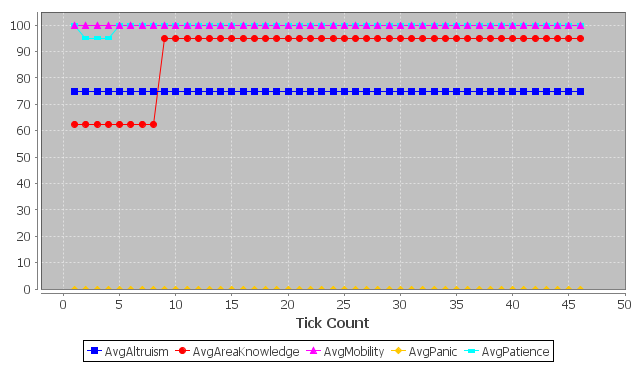
\includegraphics{directions_test.png}
	\caption{Variação dos atributos dos agentes do cenário.}
	\label{directions_graph}
	\end{figure}

	%----------------------------------------------------------------------------------------

\item \textbf{Pedido de Ajuda}

\textbf{Objetivo:} 
Testar o comportamento de ajuda de um agente para com outro.

Esta experiência consistiu na colocação, em posições adjacentes de um espaço pré-definido, de um agente do tipo \textit{IndependentKnowledgeable}, com um elevado nível de altruísmo, e de um agente do tipo \textit{IndependentUnknowledgeable}, com uma mobilidade reduzida.

\begin{figure}[H]
	\centering
	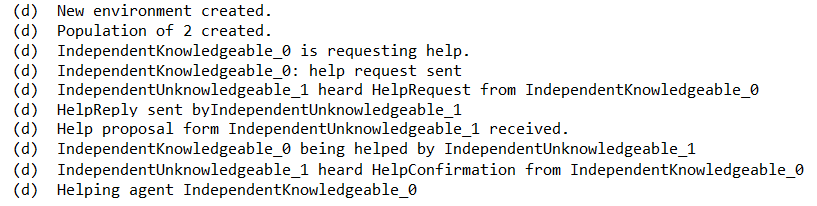
\includegraphics[scale=.8]{help_log.png}
	\caption{Excerto do registo de execução de uma simulação do cenário descrito.}
	\label{help_log}
\end{figure}

Como esperado, observou-se que o agente com mobilidade reduzida «pediu ajuda», que faz com que o outro lhe faça uma proposta. Recebendo esta proposta, o agente que efetuou o pedido envia uma confirmação, e atualiza o seu conhecimento da área com base na informação da proposta, bem como a sua mobilidade, conforme previsto para uma interação deste tipo. Na Figura \ref{help_graph} é possível verificar o aumento do conhecimento médio.

\begin{figure}[H]
	\centering
	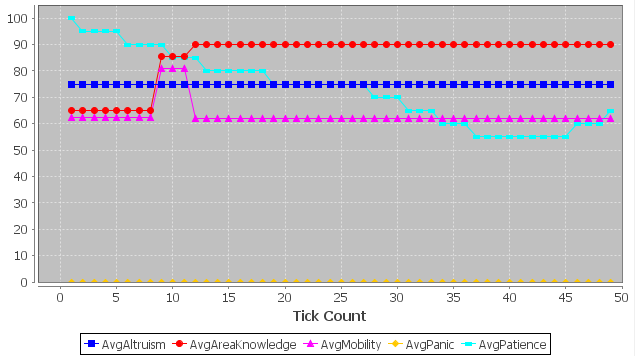
\includegraphics{help_test.png}
	\caption{Variação dos atributos dos agentes do cenário.}
	\label{help_graph}
\end{figure}
	
	De referir, ainda, que o pico na mobilidade média observado na Figura \ref{help_graph} é meramente resultado da implementação da interação, e deve-se à atualização assíncrona dos valores da mobilidade de ambos os agentes envolvidos.
%----------------------------------------------------------------------------------------
%	EXP end
%----------------------------------------------------------------------------------------
	
\end{itemize}


Terminada a fase de desenvolvimento, foram avaliados diferentes cenários.
\begin{itemize}
	\item diferentes configurações para o local do acidente, variando o número e localização de saídas de emergência e obstáculos;
	\item diferentes combinações de agentes a evacuar, variando o seu tipo, número e localização.
\end{itemize}

Deste modo, foi possível observar-se como estas variações se refletem em métricas como o tempo médio e máximo de evacuação ou o número de feridos.

\newpage
\section{Conclusão}

Terminado o projeto, destaca-se a importância de ferramentas de simulação de evacuação - perante os desafios que a realização de simulacros coloca - e a aplicabilidade deste projeto a esse fim.

Consideram-se atingidos os objetivos definidos: desenvolver um programa que permita simular a interação de agentes confinados a um espaço concreto e limitado perante a necessidade de evacuar esse espaço.

Tem-se como particularmente útil a possibilidade de acompanhar a evacuação visualmente e a possibilidade de analisar os dados recolhidos, por um lado, através de gráficos e, por outro, através do registo de eventos.

Da análise dos resultados das experiências levadas a cabo

\section{Melhorias}

Considera-se que uma possível melhoria, seria a introdução de obstáculos dinâmicos no espaço, como os elementos fumo e fogo. Tal poderia ser implementado, por exemplo, usando um agente com a capacidade de se replicar ao longo do tempo para posições adjacentes, simulando a propagação de um incêndio. Agentes na proximidade poderiam sufocar ou queimar-se, vendo a sua mobilidade reduzida ou mesmo morrer.

Outra melhoria que poderia ser introduzida passaria pela criação de um novo tipo de agente, cuja única função seria coordenar a evacuação, ajudando aqueles que precisassem de ajuda a chegar à saída. Estes agentes de segurança poderiam existir em qualquer número e deveriam coordenar-se entre si, por modo a garantir que o espaço era evacuado, i.e., que todas as pessoas (vivas) chegavam à saída.



\section{Recursos}
\subsection{Bibliografia}
[1] Almeida, João; Rosseti, Rosaldo; Coelho, António: \textit{Crowd Simulation Modeling Applied to Emergency and Evacuation Simulations using Multi-Agent Systems}. 2011.

[2] \textit{FIPA: FIPA Specification}. Disponível online em \url{http://www.fipa.org/specs/fipa00037/SC00037J.pdf}. Consultado em novembro de 2016.

[3] \textit{Respast: Repast Simphony Documentation}. Disponível online em \url{http://repast.sourceforge.net/docs/api/repast_simphony/index.html}. Consultado em novembro de 2016.

[4] \textit{SAJaS: SAJaS Documentation}. Disponível online em \url{https://web.fe.up.pt/~hlc/doku.php?id=sajas}. Consultado em novembro de 2016.


\subsection{Software}
[1] \textit{Repast Simphony};

[2] \textit{JADE};

[3] \textit{SAJaS}.

[4] \textit{Eclipse};

\newpage
%----------------------------------------------------------------------------------------
%	UserMan Begin
%----------------------------------------------------------------------------------------

\section{Apêndice}


\subsection{Manual de Utilizador}

\subsubsection{Especificação do mapa}

O ficheiro que especifica o espaço de simulação deverá ter como conteúdo um conjunto de linhas, todas com comprimento idêntico, compostas pelos caracteres \textit{'W'} - que representa uma parede, ou, mais genericamente, um obstáculo -, \textit{'E'} - que representa uma saída - e {' '}, que caracteriza um espaço livre. A ordem dos caracteres nas linhas, e das linhas no ficheiro, é a ordem considerada para a representação do mapa no ambiente na simulação.

O ficheiro poderá ser selecionado na \textit{GUI} do \textit{Repast}, através do separador \textit{Parameters} na barra lateral, colocando o endereço para o ficheiro na caixa designada \textit{Environment File Name}.

\subsubsection{Especificação do cenário}

O ficheiro que especifica a população a usar na simulação é um ficheiro .xml, e permite configurar tanto factores como atributos dos vários agentes a evacuar:
\begin{lstlisting}
<scenario 
panicVariation="INT"
mobilityVariation="INT"
knowledgeAcquisitionFactor="DOUBLE"
patienceVariation="INT"
patienceThreshold="INT"
>
	<person>
		<areaKnowledge>INT</areaKnowledge>
		<altruism>INT</altruism>
		<independence>INT</independence>
		<patienceVariation>INT</patienceVariation>
		<mobility>INT</mobility>
		<panic>INT</panic>
		<age>INT</age>
	</person>
</scenario>
\end{lstlisting}

O ficheiro poderá ser selecionado na \textit{GUI} do \textit{Repast}, através do separador \textit{Parameters} na barra lateral, colocando o endereço para o ficheiro na caixa designada \textit{Scenario File Name}.

\subsubsection{Utilização}

Após a especificação do mapa e cenário a utilizar, é conveniente, para efeitos de visualização, alterar o parâmetro \textit{Schedule Tick Delay}, através do separador \textit{Run Options}. Nas experiências utilizadas, utilizaram-se \textit{delays} de valor entre 30 a 60.

Concluído este passo, pode dar-se início à simulação, do mesmo modo que seria iniciada uma qualquer simulação \textit{Respast}.

Além de se poder acompanhar a evacuação visualmente, através de um \textit{display} do espaço e pessoas a evacuar, é possível acompanhar e analisar a evolução do processo, através de um gráfico que monitoriza o valor médio de alguns dos atributos definidos para os agentes, e de um outro gráfico, que regista o número de evacuados e mortos. Adicionalmente, é possível observar o registo da execução, que mostra mensagens relevantes para compreender algumas das interações observadas.

\end{titlepage}
\end{document}